%------------------------------------------------------------------
%
% Vorlage für Abschlussarbeiten an der Technischen Hochschule Ingolstadt
% Bachelorarbeit/Masterarbeit
%
% Angepasst auf Seminararbeit
%
% V1 05.12.2011		Dr. Paul Spannaus
% V2 07.07.2012		Dr. Paul Spannaus
% V3 10.03.2013		Dr. Paul Spannaus
% V4 28.01.2014		Dr. Paul Spannaus
% V5 31.10.2014 		Dominik Schlecht
% 	
% -----------------------------------------------------------------
% -----------------------------------------------------------------

% Dokumentenklasse
\documentclass[a4paper,11pt,DIV=11,oneside]{scrartcl} % 

% Packages
%Datum und Uhrzeit
\usepackage{datetime}

%Encoding
\usepackage[utf8]{inputenc}
\usepackage{lmodern}

%Graphikpakete
\usepackage{graphicx}
\usepackage{xcolor}
\usepackage{tikz}
\usetikzlibrary{arrows, snakes, backgrounds}
\usepackage{wrapfig}

% Farben der THI
\definecolor{THIblue}{rgb}{0.0078,0.1176,0.4705}

\usepackage[ngerman]{babel}

%Zitierumgebung
%\usepackage{cite}% Zitieren
%\usepackage[backend=biber,]{biblatex}
%\usepackage{bibgerm}% Literatur in Deutscher DIN
\usepackage[babel,german=quotes]{csquotes}
\bibliography{ref/ref_liste} % Pfad und Datei der Ref-Datenbank

%URL-Umgebung
\usepackage{url}
\renewcommand{\UrlFont}{\small\tt\color{THIblue}}

%Mathematik
\usepackage{amsmath}
\usepackage{amssymb}
\usepackage{mathtools}

%Quellcode
\usepackage{listings}
\lstset{literate=%
    {Ö}{{\"O}}1
    {Ä}{{\"A}}1
    {Ü}{{\"U}}1
    {ß}{{\ss}}1
    {ü}{{\"u}}1
    {ä}{{\"a}}1
    {ö}{{\"o}}1
    {~}{{\textasciitilde}}1
}

\definecolor{gray}{rgb}{0.5, 0.5, 0.5}
\lstset{% general command to set parameter(s)
	basicstyle=\tiny\ttfamily,%\small, % print whole listing small
	keywordstyle=\color{THIblue}\bfseries\underbar,% underlined boldblack keywords
	identifierstyle=, % nothing happens
	commentstyle=\color{green}, % white comments
	stringstyle=\color{red}\ttfamily, % typewriter type for strings
	showstringspaces=false, % no special string spaces
	%numbers=left,
	%numberstyle=\color{gray},
	%numbersep=5pt,
	captionpos=b,
	breaklines=true}
	
% Define Language
\lstdefinelanguage{log}
{
  % list of keywords
  morekeywords={
    idVendor,
    idProduct,
    bInterfaceClass,
    bInterfaceSubClass,
    bInterfaceProtocol
  },
  sensitive=false, % keywords are not case-sensitive
  %alsodigit={0482},
  morecomment=[l]{//}, % l is for line comment
  morecomment=[s]{/*}{*/}, % s is for start and end delimiter
  morestring=[b]" % defines that strings are enclosed in double quotes
}

\lstdefinelanguage{tikz}
{
  % list of keywords
  morekeywords={
	above,
	align,
  	begin,
	below,
  	caption,
	draw,
	end,
	every,
	fill,
	label,
  	line,
	minumum,
	node,
	rectangle,
	right,
	scale,
	size,
  	style,
	of,
  	width,
  	xshift,
  	yshift
  },
  sensitive=false, % keywords are not case-sensitive
  %alsodigit={0482},
  keywordstyle=\color{THIblue}\bfseries,
  morecomment=[l]{//}, % l is for line comment
  morecomment=[s]{/*}{*/}, % s is for start and end delimiter
  morestring=[b]" % defines that strings are enclosed in double quotes
}

%Microtypographie
\usepackage{microtype}

%Kopf und Fußzeilen
\usepackage{scrpage2} 	% Kopf & Fußzeile im KOMA Stil
\pagestyle{scrheadings}	% Aktiviert Verwendung vordefinierter Kolumnentitel
\clearscrheadfoot 		% alle Standard-Werte und Formatierungen löschen
\setkomafont{pagehead}{\scshape}	% Schriftart in Kopfzeile, \scshape = Kapitelchen
\automark[chapter]{section} % [linke Seite]{rechte Seite}
%\ohead{\def\pagestyle{PDTS}{\hrulefill
\includegraphics[width = 6cm]{bilder/thi_logo_quer_cropped}}}
\ohead{
\includegraphics[width = 6cm]{bilder/thi_logo_quer_cropped}}

%\ihead{\textsc{Abschlussarbeit}}
\ihead{\headmark}

%\setheadwidth[0pt]{textwithmarginpar}
\ofoot{\vspace{-0.3cm} \pagemark} 						
\ifoot{\vspace{-0.3cm} Dominik Gunther Florian Schlecht} 
				
%\setheadtopline{.4pt}				
\setheadsepline{.2pt}
\setfootsepline{.4pt}	% Trennlinie Fußzeile und Textkörper

%------------------------------------------------------------------
%% Längenanpassungen
%------------------------------------------------------------------
\setlength{\headsep}{10mm}		% Textabstand zur Kopfzeile
\setlength{\footskip}{15mm}		% Abstand zur Fußzeile
\setlength{\parindent}{0em}		% Einzug nach Absatz

%%-------------Allgemeine Definitionen----------------------------------
% Farbige Aufwertung der berschriften
\addtokomafont{chapter}{\color{THIblue}}
\addtokomafont{section}{\color{THIblue}}
\addtokomafont{caption}{\color{THIblue}}
\addtokomafont{subsection}{\color{THIblue}}
\addtokomafont{subsubsection}{\color{THIblue}}
\setkomafont{captionlabel}{\color{THIblue}}

%Hyperref
\usepackage[
		pdftex,
		linkcolor=THIblue,			% Farbe der Verlinkung
		linktocpage=true,			% Im TOC wird Seitenzahl verlinkt(true),bzw. Text(false)
		colorlinks=true,			% 'true' keinen Kasten um Link
		citecolor=THIblue,
%		pdfhighlight=/P,
%		bookmarks,
%		hyperfigures=true,
%		citebordercolor={0 0 1},
%		linkbordercolor={0 0 1},
%		menubordercolor={0 0 1},
%		backref=true,
%		pagebackref=true,
%		bookmarksopen,
%		bookmarksnumbered,
%		pdfpagelabels=false,
%		pdfstartpage=1,
%		pdfstartview=Fit,			% Modus beim Öffnen (Fit = An Seitengröße anpassen)
		pdftitle={Umgehen von USB-Deskriptor basierten USB-Policies am Beispiel einer virtuellen Umgebung},
		pdfauthor={Dominik Schlecht},
%		pdfstartview=Fit,
%		pdfdisplaydoctitle=true,
%		plainpages=false
			]{hyperref}  

%------------------------------------------------------------------
% Wichtige Definition für Aufteilung von Formelverzeichnis und Abkürzungsverzeichnis
%------------------------------------------------------------------

% Nomenklaturverzeichnis, Formelzeichenliste Anpassungen für nomenclature: damit lassen sich zwei getrennte Symbolverzeichnisse anlegen, ziehmlich cool!
\usepackage[intoc,compatible,german]{nomencl}	
		\renewcommand{\nomgroup}[1]{	\ifthenelse{\equal{#1}{A}}{\item[{\normalfont\sffamily\bfseries\LARGE\textcolor[rgb]{0,0.112,0.47}{Abkürzungen{\phantom{\Huge $\frac{\frac{\frac{A}{a}}{a}}{\frac{a}{a}}$}}}}]}{	\ifthenelse{\equal{#1}{A}}{\item[{\normalfont\sffamily\bfseries\LARGE\textcolor[rgb]{0,0.112,0.47}{Formelzeichen{\phantom{\Huge $\frac{A}{\frac{a}{a}}$}}}}]}{}}}
		
%------------------------------------------------------------------
%% Anpassung von Abständen, Längen vom Nomenclaturverzeichnis (Abkürzungs- und Formelverzeichnis)
%------------------------------------------------------------------

% Abstand zwischen Einträgen im Symbolverzeichnis (-\parsep = 0)
\setlength{\nomitemsep}{-\parsep} 
\setlength{\nomlabelwidth}{5em}	
\renewcommand{\nomlabel}[1]{#1 \dotfill}  % Punkte im zwischen Nummer und Kapiteleintrag


%%-------------Silbentrennung--------------------------------------
\hyphenation{}

%%-------------Index-----------------------------------------------
\makeindex

%-----------------------------------------------------------------
%---------------Dokumentenbeginn----------------------------------
%-----------------------------------------------------------------
\begin{document}
	
% Titelseite
\begin{titlepage}

\phantom{tmpText}

\vspace{1cm}

\begin{figure}[h!]
\centering

\includegraphics[width=\textwidth]{bilder/thi_logo_cropped.pdf}
\end{figure}

  \begin{center}

%\vspace{1cm}
    
    
    \textbf{{\large Seminararbeit/Whitepaper} \\[3ex]
    {\LARGE Malwareanalyse} \\[1ex]
    %
    \vfill
    %
    angefertigt von} \\
    \begin{tabular}{ll}
    	Name: & Dominik Gunther Florian Schlecht\\
    	Matrikelnummer: & 00032209\\[2ex]
    	\multicolumn{2}{c}{\textbf{Betreuer:}}\\
    	Technische Hochschule Ingolstadt: & Prof. Hahndel
    \end{tabular}\\[2ex] %Vorname Nachname
    %
    \vfill
    %
    Ingolstadt, \today
  \end{center}
\end{titlepage}

	\pagenumbering{roman} % Nummerierung
	%\include{chapter/thanks_statement}
	\tableofcontents % Inhaltsverzeichnis
	\newpage
%---------------Hauptteil-----------------------------------------
	\pagenumbering{arabic} 	% Neunummerierung des Hauptteils
	\setcounter{page}{0}	% Wieder bei 1 Anfangen
	\chapter{Einleitung}
TODO	
	\section{Verwendete Tools und Infrastruktur}
	\subsection{Physikalisches Betriebssystem}
Als Grundsystem wurde ein Linux verwendet. Dies hat den Vorteil, dass ein Großteil der sich derzeit im Umlauf befindlichen Malware für Windows konzipiert ist. (Ebenso steigt der Anteil der Malware für mobile Betriebssysteme stetig, diese werden hier jedoch nicht behandelt.) Als unkompliziertes, wandelbares und trotzdem hoch modifizierbares System wurde Debian 8 gewählt. Versuche mit z.B. Gentoo zeigten Probleme mit der verwendeten Virtualisierungslösung. 

\subsection{Virtualisierungslösung}
Es gibt viele Vorteile für die Nutzung einer Virtualisierungslösung bei der Malwareanalyse, jedoch auch Nachteile. Vorteilhaft ist vor allem das erstellen von sogenanneten Snapshots, welche einen bestimmten Zustand eines Systems aufzeichnen und es möglich machen, diesen später wieder herzustellen. Zudem wird das Host-System vor der Malware geschützt. Ein Nachteil ist, dass moderne Malware immer häufiger überprüft, ob sie in einer virtuellen Umgebung ausgeführt wird. Falls ja, werden oft andere Funktionen ausgeführt, um die ursprüngliche Funktion zu verschleiern. Insgesammt überwiegen aber die Vorteile den Nachteil. Falls die Malware auf die virtuelle Umgebung prüft, muss geprüft werden, ob über Prüffunktion über den Disassembler deaktiviert oder umgangen werden kann.

Als Virtualisierungslösung wurde VMWare Workstation 11 genutzt. Diese bietet gerade im Bereich der Netzwerkmodifikation weitere Möglichkeiten gegenüber der kostenlosen Variante Virtualbox von Oracle. Die Workstation kann von der offiziellen Webseite heruntergeladen und für 30 Tage kostenlos getestet werden.

\subsection{Virtuelles Betriebssystem}
Als virtuelles Betriebssystem wurde Windows 7 Pro verwendet. Dies ergibt sich einfach daraus, dass Windows 7 derzeit mit eines der meistverbreiteten Betriebssysteme ist und Malware meistens für Windows konzipiert ist.

Zudem wurde 32-bit als Architektur gewählt, um die Komapatibilät mit Tools wie Cukoo siche zu stellen. Außedem wurden sowohl das UAC, Updates sowie die Firewall deaktiviert, um der Malware eine Möglichst einfache Umgebung zu bieten. Die VMWare-Tools wuden absichtlich nicht installiert, da dies einer Malware eine sehr einfache Möglichkeit bieten würde, die Umgebung zu erkennen.

Diese Konfiguraton wird als Grundimage verwendet.

\subsection{Disassembler}
Als Disassembler wurde IDA PRO Free (Version 5.0) verwendet. Diese Version reicht für grundliegende Analysen, jedoch sind die möglichen Anwendungen auf 32-bit begrenzt. Da Malware jedoch so konzipiert ist, dass ein möglichst breites Spektrum an Geräten angegriffen werden kann, ist diese zumeist ebenfalls 32-bit. Um mit IDA PRO Free 64-bit Malware zu analysieren, ist eine kostenpflichtige Version notewendig. Als Alternative zu IDA PRO Free kann Hopper in Betracht gezogen werden. Hopper gibt es ebenfalls in einer kostenfreien Version, die Stärke liegt jedoch in der kostenpflichtigen Lizenz, welche ähnliche Features bietet wie IDA PRO, jedoch wesentlich billiger und somit auch für Privatpersonen erschwinglich ist. Zudem bietet Hopper den Vorteil, dass es vorgefertige Versionen für Windows, OS X und Linux gibt. IDA Pro (Free) liegt nur für Windows vor, ist jedoch über Wine relativ einfach auf Linux installierbar.

\subsection{Weitere Tools}
\subsubsection{RegShot}
\subsubsection{Resoucehacker}
\subsubsection{PEView}
\subsection{Webseitn}
\subsubsection{Virustotal}
\subsubsection{Malwr}
	\section{Infektionsweg}
	\section{Dynamische Analyse}
	\section{Statische Analyse}
	\section{Fazit}
%---------------Anhang-------------------------------------------
	
%------------------------------------------------------------------------
% Anhänge
\appendix
\section{Appendix}
\subsection{Version Info}
\label{ref:versionInfo}
\begin{lstlisting}
1 VERSIONINFO
FILEVERSION 1,1,1,1
PRODUCTVERSION 1,1,1,1
FILEOS 0x4
FILETYPE 0x1
{
BLOCK "StringFileInfo"
{
	BLOCK "040904b0"
	{
		VALUE "CompanyName", "Valve"
		VALUE "FileDescription", "Half-Life Launcher"
		VALUE "FileVersion", "1, 1, 1, 1"
		VALUE "InternalName", "Half-Life Launcher"
		VALUE "LegalCopyright", "Copyright (c) 1996-2003"
		VALUE "LegalTrademarks", ""
		VALUE "OriginalFilename", "hl.exe"
		VALUE "ProductName", "Half-Life Launcher"
		VALUE "ProductVersion", "1, 1, 1, 1"
	}
}

BLOCK "VarFileInfo"
{
	VALUE "Translation", 0x0409 0x04B0
}
}
\end{lstlisting}

\newpage
\subsection{Abbildungen}

\begin{figure}[htbp]
	\centering
	
\includegraphics[scale=0.5]{bilder/EMail.png}
	\caption{Gefälschte UPS-Mail}
	\label{img:EMail}
\end{figure}

\begin{figure}[htbp]
	\centering
	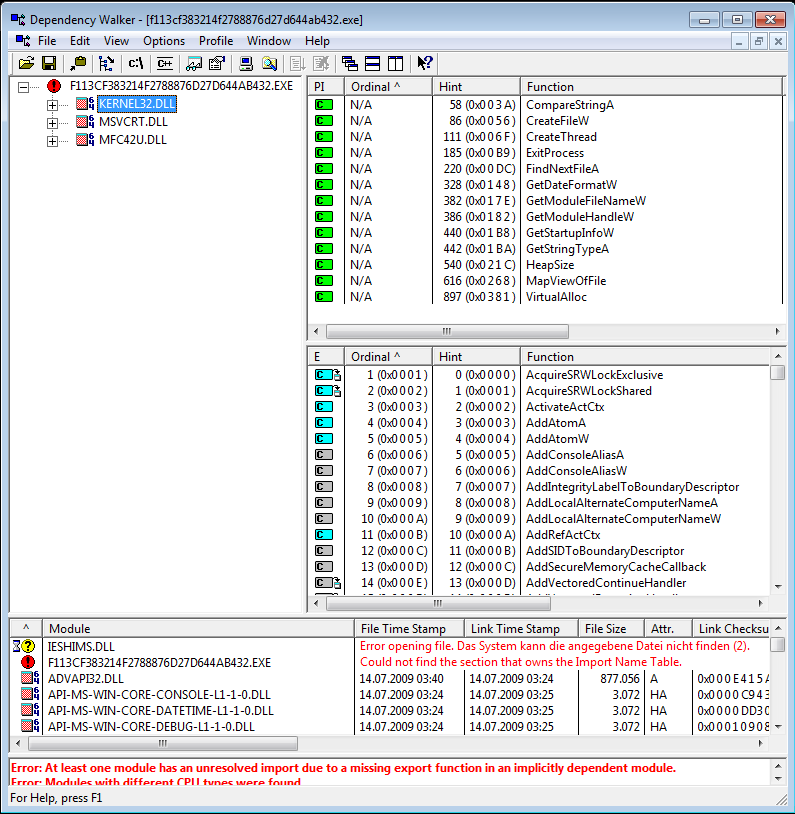
\includegraphics[scale=0.5]{bilder/statischeAnalyse/depWalker.png}
	\caption{Aufruf der Datei \textit{f113} mit dem Dependency Walker}
	\label{img:depWalkerf113}
\end{figure}

\begin{figure}[htbp]
	\centering
	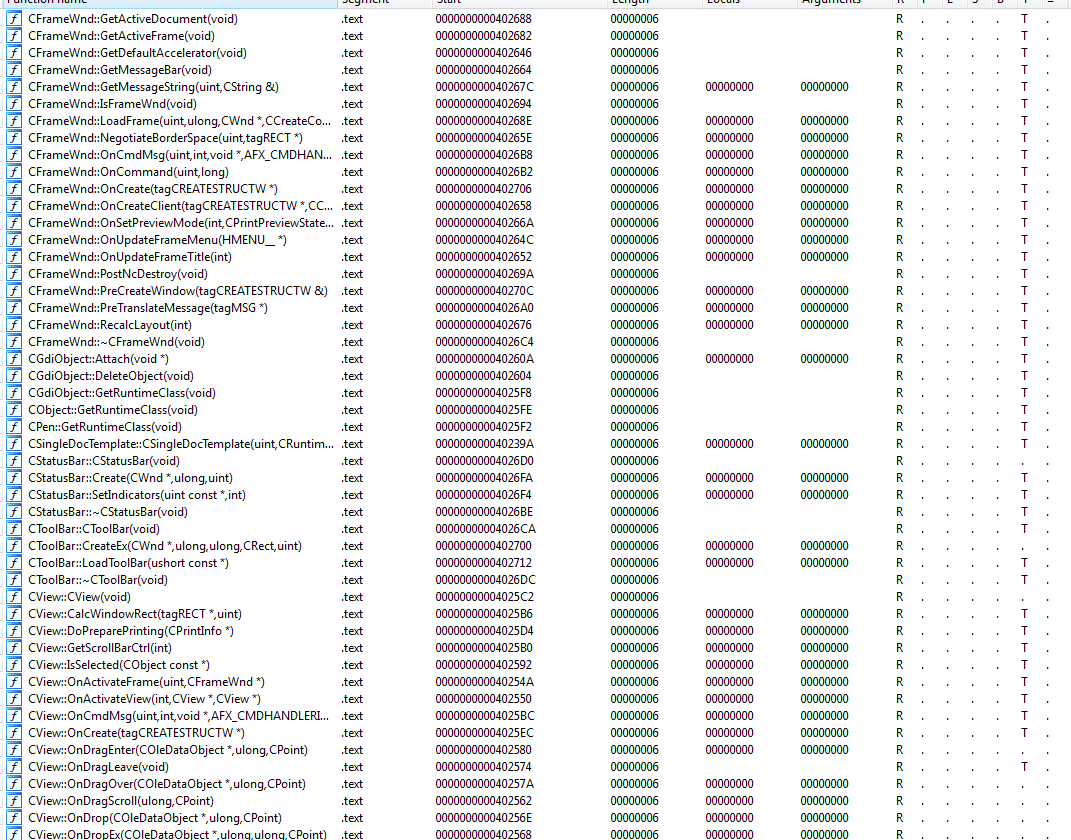
\includegraphics[width=\textwidth]{bilder/statischeAnalyse/IDAFunc.png}
	\caption{Funktionsaufrufe der Datei \textit{f113}, Ansicht in IDA}
	\label{img:IDAFuncf113}
\end{figure}

\begin{figure}[htbp]
	\centering
	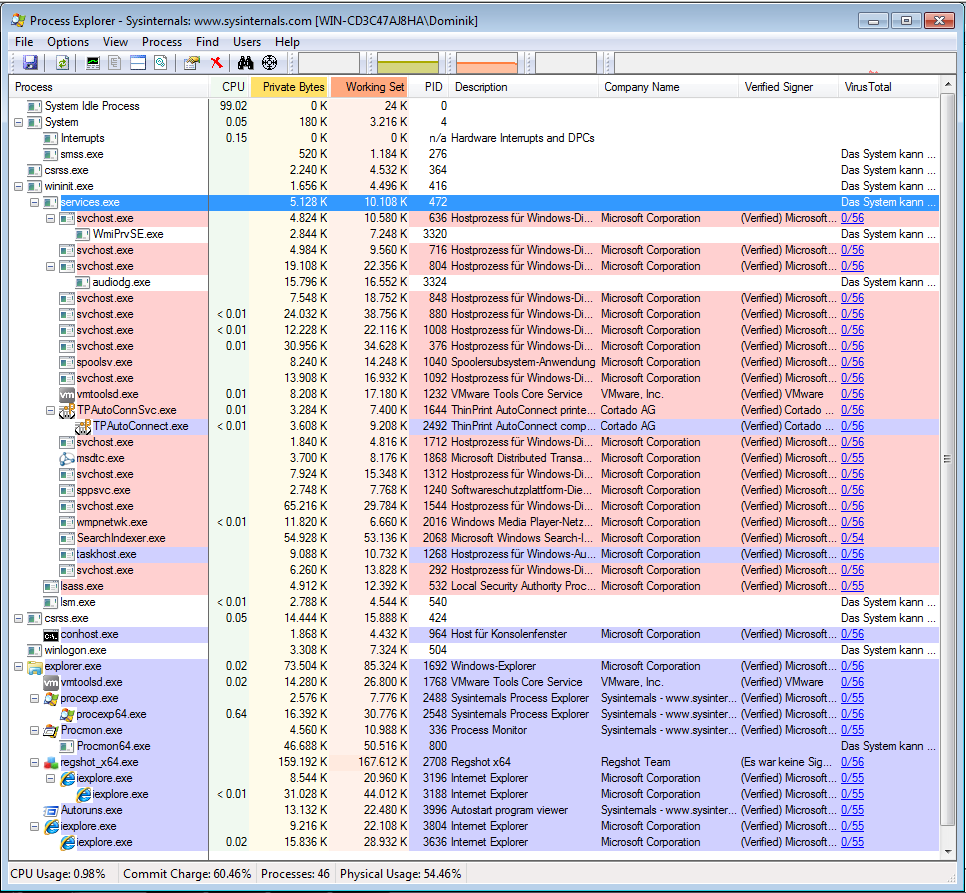
\includegraphics[width=\textwidth]{bilder/dynamischeAnalyse/ProcessExplorer.png}
	\caption{Process Explorer nach Ausführung von \textit{f113} mit Abgleich der Prozesse mit Virustotal}
	\label{img:ProcExpf113}
\end{figure}

\begin{figure}[htbp]
	\centering
	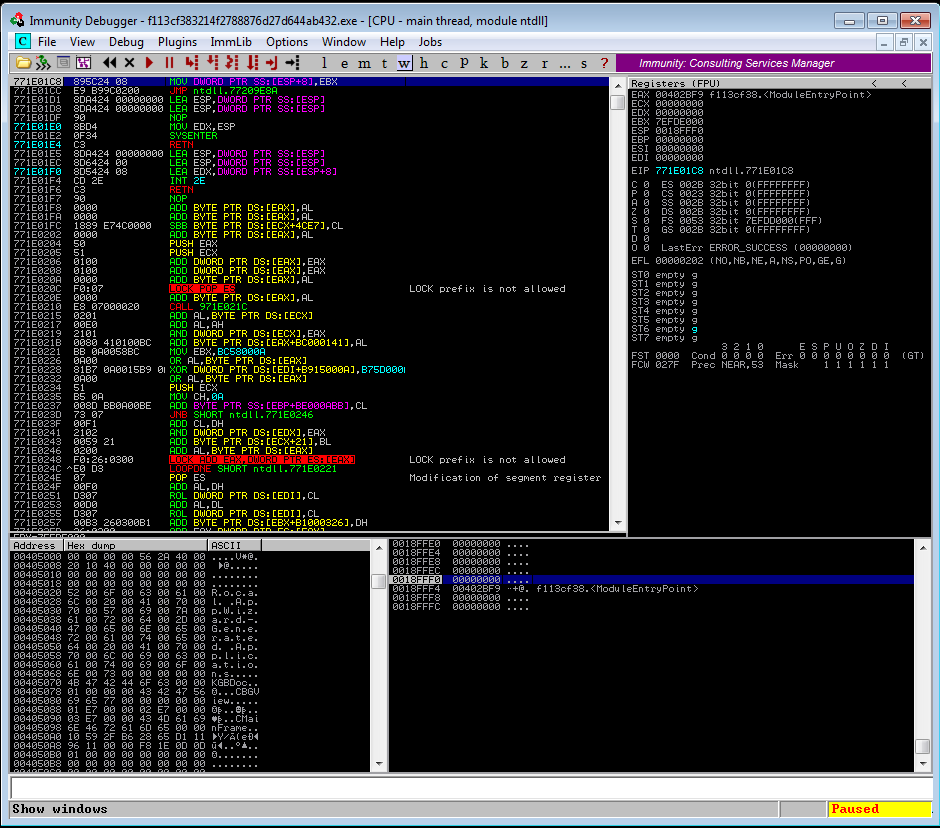
\includegraphics[width=\textwidth]{bilder/dynamischeAnalyse/ImmunityDebug.png}
	\caption{Hauptfenster des \textit{Immunity Debuggers} nach Ausführung von \textit{f113}}
	\label{img:ImmunityDebf113}
\end{figure}

\begin{figure}[htbp]
	\centering
	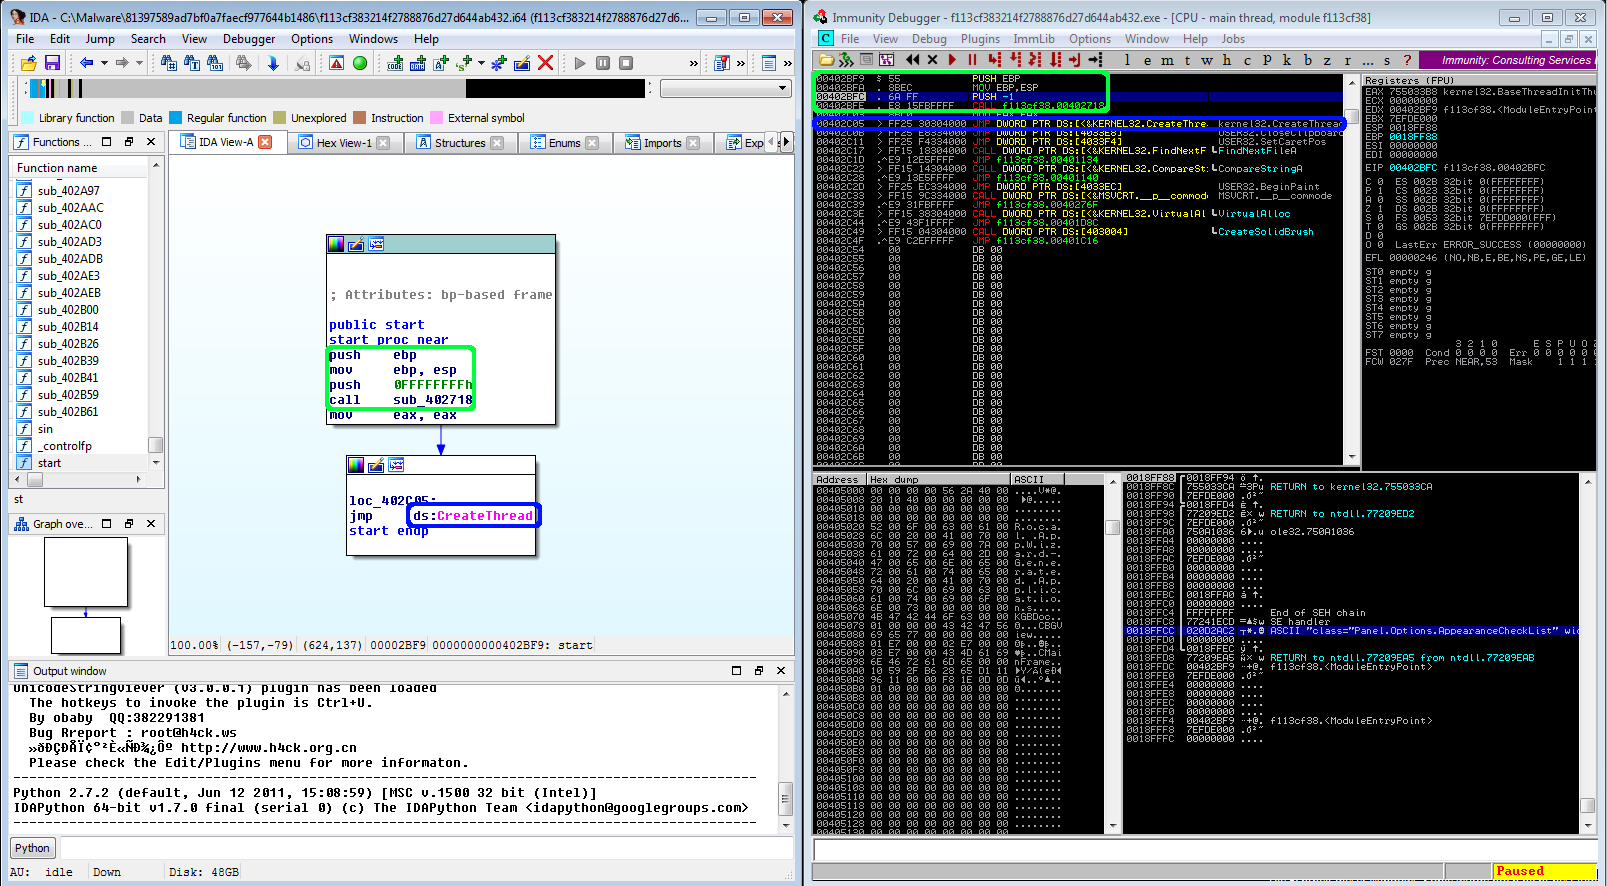
\includegraphics[angle=90, scale=.35]{bilder/dynamischeAnalyse/IDAtoImmunity.png}
	\caption{Zusammenhang von \textit{IDA} und \textit{Immunity Debuggers} bei \textit{f113}}
	\label{img:IDAtoImmunityf113}
\end{figure}

\begin{figure}[htbp]
	\centering
	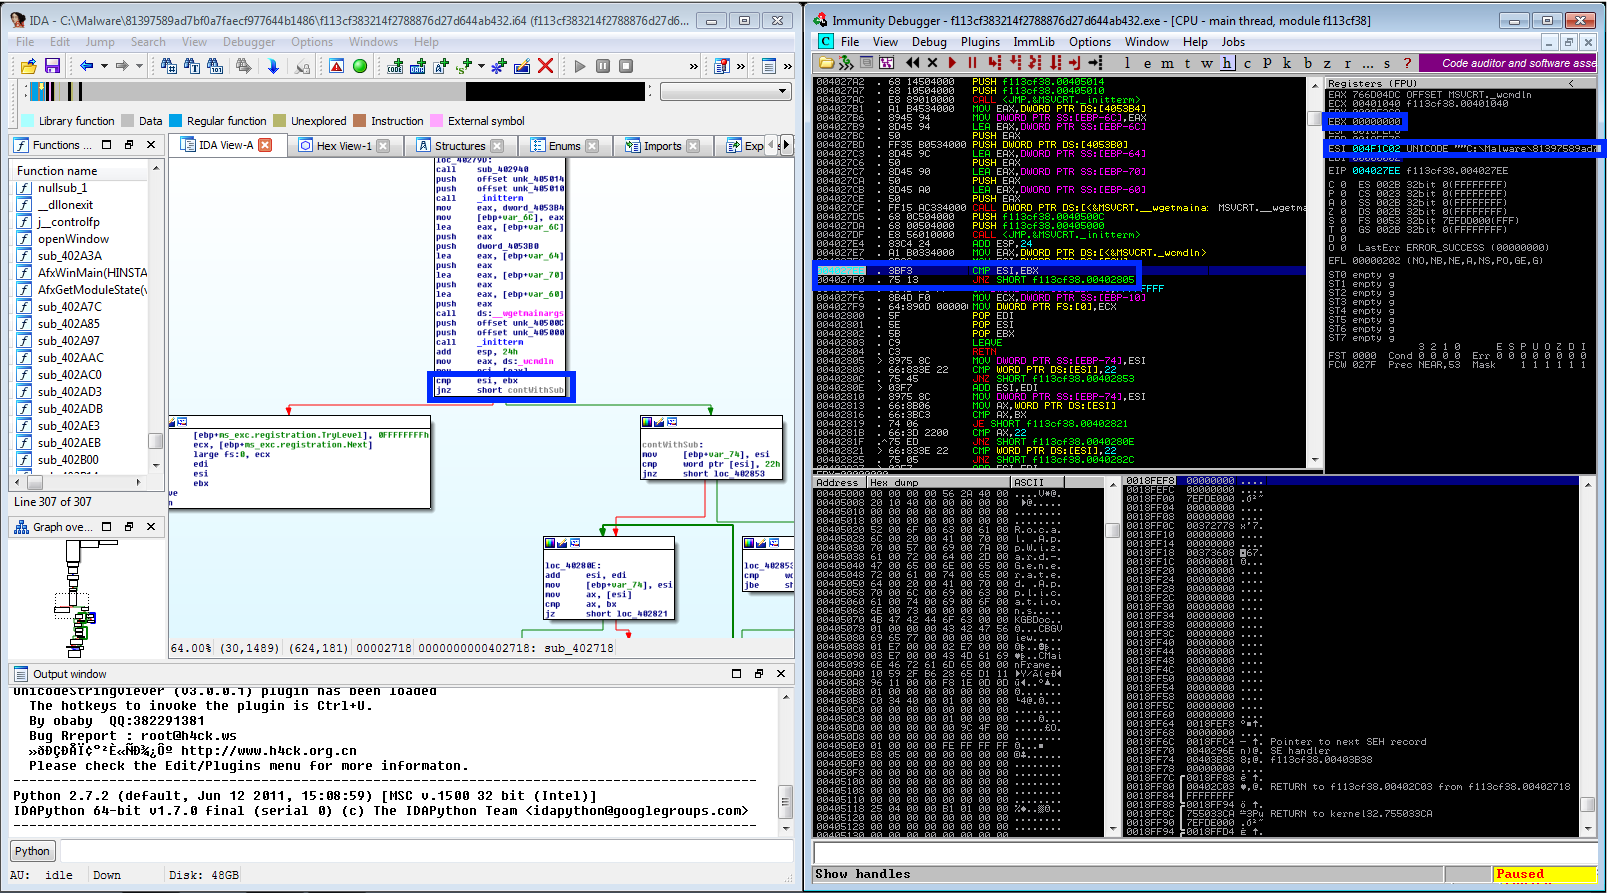
\includegraphics[angle=90, scale=.35]{bilder/dynamischeAnalyse/IDAtoImmunity2.png}
	\caption{Zusammenhang von \textit{IDA} und \textit{Immunity Debuggers} bei \textit{f113}}
	\label{img:IDAtoImmunity2f113}
\end{figure} % Anhang
	\newpage
%	\printbibliography % Literaturliste
\end{document}
%-----------------------------------------------------------------
%---------------Dokumentenende------------------------------------
%-----------------------------------------------------------------
